\documentclass{beamer}
\usepackage[orientation=portrait,width=30in,height=40in,scale=1.35,debug]{beamerposter}
\mode<presentation>{\usetheme{ZH}}
\usepackage{chemformula}
\usepackage[utf8]{inputenc}
\usepackage[english]{babel} % required for rendering German special characters
\usepackage{hyperref} %enable hyperlink for urls
\usepackage{ragged2e}
\usepackage[font=small, justification=justified]{caption}
\usepackage{array,booktabs,tabularx}
\usepackage{bm}
\usepackage{subcaption}

\def\ci{\perp\!\!\!\!\!\perp}

\newcolumntype{Z}{>{\centering\arraybackslash}X} % centered tabularx columns
\title{\huge A Simple Unified Approach to Testing High-Dimensional Conditional Independencies for Ordinal and Categorical Variables}
\author{Ankur Ankan, Johannes Textor}
\institute[RU]{Institute for Computing and Information Sciences \\ Radboud University, Netherlands}
\date{\today}

% edit this depending on how tall your header is. We should make this scaling automatic :-/
\newlength{\columnheight}
\setlength{\columnheight}{106cm}

\begin{document}
\begin{frame}
\begin{columns}
	\begin{column}{.33\textwidth}
		\begin{beamercolorbox}[center]{postercolumn}
			\begin{minipage}{.98\textwidth}  % tweaks the width, makes a new \textwidth
				\parbox[t][\columnheight]{\textwidth}{ % must be some better way to set the the height, width and textwidth simultaneously
	\begin{myblock}{Introduction}
		\begin{figure}
			\begin{subfigure}{0.4\textwidth}
				\centering
				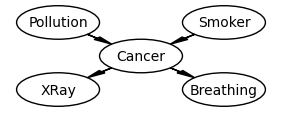
\includegraphics[scale=1.5]{../in_person/imgs/example_dag.png}
			\end{subfigure}\hfill%
			\begin{subfigure}{0.1\textwidth}
				$$ \bm{\implies} $$
			\end{subfigure}\hfill%
			\begin{subfigure}{0.5\textwidth}
				\begin{equation*}
					\begin{split}
						\text{\emph{XRay}} \ci \text{\emph{Pollution}}  &| \text{\emph{Cancer}} \\
						\text{\emph{Breathing}} \ci \text{\emph{Smoker}} &| \text{\emph{Cancer}} \\
						\cdot \cdot \cdot & \\
					\end{split}
				\end{equation*}
			\end{subfigure}
			\caption*{Causal Markov Condition in a DAG \footnotemark}
		\end{figure}
		\begin{itemize}
			\item \justifying In applied research, most of the DAGs are constructed by
				hand based on domain knowledge. Hence, it is crucial 
				to test whether the theorized model is consistent with
				the data. Conditional Independence (CI) tests can be
				used to test these models by verifying whether the
				implied CIs of the model are valid in the data or not.
			\item \justifying Constraint-Based structure learning algorithms like PC and FCI systematically search
				for CIs in data to construct the model skeleton. They start with
				a fully connected network and iteratively remove edges if the variables 
				are (conditionally) independent given some of their neighbours.
				% CI implies that no direct causal link exists between the variables.
				% $$ \text{\emph{XRay}} \ci \text{\emph{Smoker}} | \text{\emph{Cancer}} \implies \text{No edge b/w \emph{XRay} and \emph{Smoker}} $$
		\end{itemize}

	\end{myblock}\vfill
	\begin{myblock}{Current Approaches to CI Testing}
		\justifying \textbf{Stratification tests:} Converts a CI
				test into a set of non-conditional independence
				tests by splitting the dataset into smaller
				datasets corresponding to every possible value
				of conditional variables and combines
				the results. This is the most common approach
				for discrete variables. The main drawback is
				that tests lose power quickly as the number
				of conditional variables increases. E.g.,
				Chi-Squared test, G-test. \\
				\vspace{0.8em}
		\justifying \textbf{Variable Importance tests:} Based
				on comparing the ``goodness of fit'' of two
				estimators: $ \hat{p}(x | y, z) $ and $
				\hat{p}(x|z) $. If the simpler model does not
				fit worse, it implies that the variables are
				conditionally independent. A benefit is that
				any estimator with a goodness of fit measure
				can be used, but tests are inherently
				asymmetrical. E.g., SCCI. \\
				\vspace{0.8em}
		\justifying \textbf{Residualization tests:} Uses two
				estimators, $ \mathbb{E}[X | Z] $ and $
				\mathbb{E}[Y|Z] $, and tests for multiplicative
				association between their residuals
				\cite{Daudin1980}. Any unbiased estimator can
				be used and the tests are symmetrical. There is
				no such test for categorical/ordinal variables,
				as there is no straightforward definition of
				residuals. E.g., Generalized Covariance
				Measure(GCM), partial correlation.
	\end{myblock}\vfill
	\begin{myblock}{Proposed Residualization Based Test}
		\justifying \textbf{Estimator:} Asymptotic results require
				the estimators to be M-Estimators (e.g.,
				Generalized Linear Model (GLM)). However, in
				empirical analysis, we show that it is not a
				strict requirement. \\
				\vspace{0.8em}
		\justifying \textbf{Residuals:} We use Li-Shepherd (LS) residuals \cite{li2012}.
				Given an ordinal variable $ Y $ and an estimate $ \hat{p}(y) $ of $
				p(y) $, LS-Residual for sample $ y_i $ is defined as:
				$$ R_{y_i} = \hat{p}(Y < y_i) - \hat{p}(Y > y_i) $$

				For the binary case with $ Y \in \{0, 1\} $:
				$$ R_{y_i} = y_i - \hat{p}(Y = 1) $$

				For the conditional case for sample $ (y|z)_i $,
				$$ R_{y_i | z_i} = \hat{p}(Y < y_i | Z=z_i) - \hat{p}(Y>y_i|Z=z_i) $$ \\
				\vspace{0.8em}
		\justifying \textbf{Test Statistic:} Hotelling's $ T^2 $ test
				(a multidimensional location test) on residual
				products.
	\end{myblock}\vfill
	\begin{myblock}{Test Statistic}
		\begin{itemize}
			\item \textbf{Both Ordinal Variables:}
			$$ Q_1(\bm{x}, \bm{y}) = \frac{1}{n} \frac{(R_{\bm{x}} \cdot R_{\bm{y}})^2}{\bm{var}(R_{\bm{x}} R_{\bm{y}})} $$
			If $ X \ci Y | Z $, asymptotically $ Q_1 \sim \chi^2(1) $.
		\end{itemize}
	\end{myblock}\vfill
		}\end{minipage}\end{beamercolorbox}
	\end{column}

%%%%%%%%%%%%%%%%%%%%%%%%%%%%%%%%%%%%%%%%%%% Second Column %%%%%%%%%%%%%%%%%%%%%%%%%%%%%%%%%%%%%%%%%%%%%%%%%%%%%%%

	\begin{column}{.33\textwidth}
		\begin{beamercolorbox}[center]{postercolumn}
			\begin{minipage}{.98\textwidth} % tweaks the width, makes a new \textwidth
				\parbox[t][\columnheight]{\textwidth}{ % must be some better way to set the the height, width and textwidth simultaneously
	\begin{myblock}{Test Statistic Cont.}
		\begin{itemize}
			\item \textbf{One Ordinal and One Categorical Variable:}
						$$ Q_2(\bm{x}, \bm{y}) = \frac{1}{n} (d \times \hat{\Sigma}_d^{-1} \times d^T) $$
						$$ d = (R_{\mathbb{I}(\mathbf{x}=1)} \cdot R_{\mathbf{y}}, \, \ldots \ , R_{\mathbb{I}(\mathbf{x}=k-1)} \cdot R_{\mathbf{y}}) $$
				If $ X \ci Y | Z $, asymptotically $ Q_2 \sim \chi^2(k-1) $.
			\item \textbf{Both Categorical Variables:}
			\begin{equation*}
				\begin{split}
					& Q_3(\bm{x}, \bm{y}) = \frac{1}{n} (d \times \hat{\Sigma}_d^{-1} \times d^T) \\
				d = (&R_{\mathbb{I}(\mathbf{x}=1)} \cdot R_{\mathbb{I}(\mathbf{y}=1)}, \, \ldots \ ,
						R_{\mathbb{I}(\mathbf{x}=k-1)} R_{\mathbb{I}(\mathbf{y}=1)}, \, \ldots \, , \\
				     &R_{\mathbb{I}(\mathbf{x}=1)} \cdot R_{\mathbb{I}(\mathbf{y}=r-1)}, \, \ldots \ ,
						R_{\mathbb{I}(\mathbf{x}=k-1)} R_{\mathbb{I}(\mathbf{y}=r-1)}) 
				\end{split}
			\end{equation*}
			
			If $ X \ci Y | Z $, asymp. $ Q_3 \sim \chi^2((k-1)(r-1)) $.
		\end{itemize}

	\end{myblock}\vfill
	\begin{myblock}{Empirical Analysis}
		\begin{figure}
			\centering
			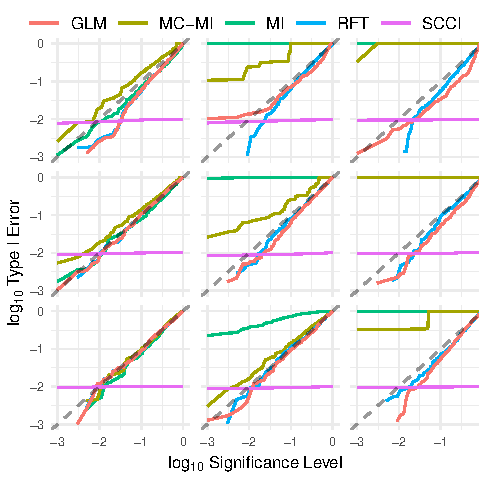
\includegraphics[scale=3]{../in_person/imgs/calibration_add_vars.pdf}
			\caption{Type I error vs significance level for sample sizes (top to
			bottom): $ [20, 40, 80] $ and number of conditional variables (left to
			right): $ [1, 3, 5] $ on conditionally independent binary datasets.}
			\label{fig:calibration}
		\end{figure}
		\begin{figure}
			\centering
			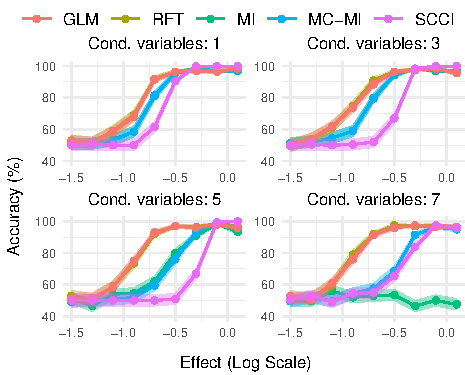
\includegraphics[scale=3]{../in_person/imgs/accuracy.pdf}
			\caption{Accuracy (shading: mean $\pm$ standard error, $N=200$) of classifying
			simulated binary datasets (sample size: $1000$) as conditionally
			dependent or independent.}
			\label{fig:cat_discrimination}
		\end{figure}
		\begin{figure}
			\centering
			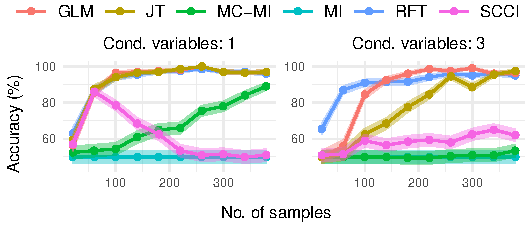
\includegraphics[scale=3]{../in_person/imgs/accuracy_ordinal.pdf}
			\caption{Accuracy (shading: mean $\pm$ standard error, N=200) of
				classifying simulated ordinal data (8 levels per variable) as
				conditionally dependent or independent.}
			\label{fig:accuracy_ord}
		\end{figure}
		\begin{figure}
			\centering
			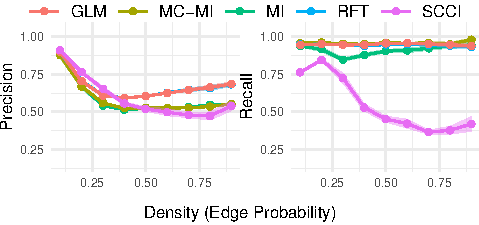
\includegraphics[scale=3]{../in_person/imgs/model_testing.pdf}
			\caption{Precision and recall of testing implied versus non-implied CIs
				 in binary data (N=1000) simulated from random DAGs on $ 20 $ variables.
				 Shading: mean $\pm$ standard error.} 
			\label{fig:model_testing}
		\end{figure}
	\end{myblock}
		}\end{minipage}\end{beamercolorbox}
	\end{column}


%%%%%%%%%%%%%%%%%%%%%%%%%% Third column %%%%%%%%%%%%%%%%%%%%%%%%%%%%%%%%%%%%%%%%%%%%%%%%%%%%%
	\begin{column}{0.33\textwidth}
		\begin{beamercolorbox}[center]{postercolumn}
			\begin{minipage}{.98\textwidth} % tweaks the width, makes a new \textwidth
				\parbox[t][\columnheight]{\textwidth}{ % must be some better way to set the the height, width and textwidth simultaneously
	\begin{myblock}{Empirical Analysis Cont.}
		\begin{figure}
			\centering
			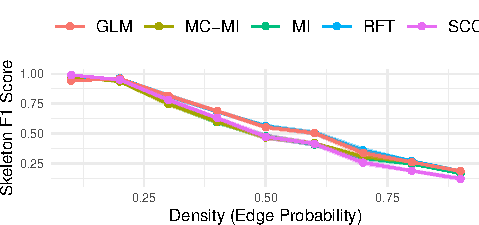
\includegraphics[scale=3]{../in_person/imgs/sl_density.pdf}
			\caption{Structure learning on simulated data: Mean F1 scores (10
				 simulated binary datasets per point) for varying graph densities. Each
				 dataset contains 1000 samples and is simulated from a randomly
				 generated DAG with 20 variables. Shading: mean $\pm$ standard error.}
			\label{fig:sl_density}
		\end{figure}
		\begin{figure}
			\centering
			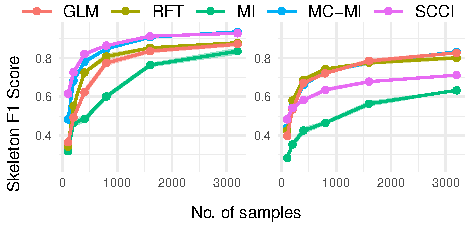
\includegraphics[scale=3]{../in_person/imgs/sl.pdf}
			\caption{Structure learning on datasets ``alarm'' (left) and ``insurance'' (right):
				Mean F1~scores (10 subsampled datasets per sample size) of the learned
				model skeletons.  Presence of an edge is considered the ``positive'' case
				for F1~scores. Shading: mean $\pm$ standard error.}
			\label{fig:sl}
		\end{figure}
		\begin{figure}
			\centering
			\begin{subfigure}[t]{0.55\textwidth}
				\centering
				\begin{tikzpicture}[scale=5]
					\tikzstyle{every node}=[inner sep=1pt, align=center]
					\scriptsize
					\begin{scope}[scale=0.2, shift={(-5cm, 0)}]
						\node at (0,0) {\footnotesize Incm};
						\node at (3,0) {\footnotesize Wrkc};
						\node at (6,0) {\footnotesize Edct};
						\node (mrts) at (9 ,0) {\footnotesize MrtS};
						
						\node at (0,-1) {\footnotesize Occp};
						\node (rltn) at (6,-1) {\footnotesize Rltn};
						\node at (3,-1) {\footnotesize Race};
						\node (sex) at (9,-1) {\footnotesize Sex};
						
						\node (hrpw) at (0,-2) {\footnotesize HrPW};
						\node at (6,-2) {\footnotesize NtvC};
						\node (age) at (3,-2) {\footnotesize Age};
						\draw [very thick] (sex) -- (rltn);
						\draw [very thick] (mrts) -- (rltn);
						\draw [very thick] (hrpw) -- (age);
					\end{scope}
					\begin{scope}[shift={(0, -2cm)}]
						\node (hrpw) at (0:1.2cm) {\footnotesize HrPW};
						\node (race) at (-33:1.2cm) {\footnotesize Race};
						\node (ntvc) at (-61:1.2cm) {\footnotesize NtvC};
						\node (edct) at (-98:1.2cm) {\footnotesize Edct};
						\node (age) at (-131:1.2cm) {\footnotesize Age};
						\node (mrts) at (-164:1.2cm) {\footnotesize MrtS};
						\node (rltn) at (-196:1.2cm) {\footnotesize Rltn};
						\node (sex) at (-225:1.2cm) {\footnotesize Sex};
						\node (occp) at (-262:1.2cm) {\footnotesize Occp};
						\node (incm) at (-300:1.2cm) {\footnotesize Incm};
						\node (wrkc) at (-333:1.2cm) {\footnotesize Wrkc};
		
						\draw [] (hrpw) -- (race) -- (ntvc) -- (edct) -- (age) -- 
							(mrts) -- (rltn) -- (sex) -- (occp) -- (incm) -- (wrkc) -- (hrpw);
		
						\draw [] (hrpw) -- (incm) -- (age) -- (hrpw);
		
						\draw [] (wrkc) -- (edct) -- (occp) -- (wrkc);
		
						\draw [] (edct) -- (rltn) -- (age);
		
						\draw [] (hrpw) -- (edct) -- (incm);
					\end{scope}
				\end{tikzpicture}
				\caption{}
				\label{fig:sl_adult_model}
			\end{subfigure}%
			\begin{subfigure}[t]{0.4\textwidth}
				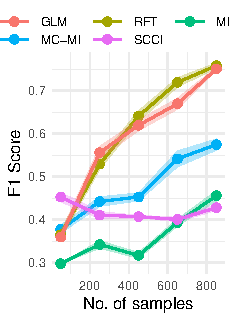
\includegraphics[scale=2.7]{../in_person/imgs/adult_F1.pdf}
				\caption{}
				\label{fig:sl_adult}
			\end{subfigure}
			\caption{Structure learning on adult income data. (a) Skeleton
				estimated by the stable PC algorithm using
				(top) Chi-Squared test (bottom) RFT (b) Mean F1
				score ($10$ adult income data subsamples per
				point) when comparing $d$-connected variable
				pairs in the CPDAG to correlated variable pairs
				in the dataset. Presence of d-connection is
				used as the positive case for the F1 score.
				Shading: mean $\pm$ standard error.}
		\end{figure}
	\end{myblock}\vfill
	\begin{myblock}{Conclusion}
		\begin{itemize}
			\item \justifying A residualization-based CI test that works for a
				combination of ordinal and categorical
				variables.
			\item \justifying Properties: 1) Simple to implement; 2)
				Interpretable chi-square test statistic; 3)
				Symmetric by construction; 4) Computationally
				feasible for structure learning applications.
			\item \justifying Performs reasonably well for low number of
				conditional variables but performs better for
				high number of conditional variables.
			\item \justifying For structure learning, a hybrid approach can be
				used with other tests.
			\item  \justifying Estimators like Random Forests can work with a
				combination of discrete and continuous
				variables, and hence we can possibly extend to
				a single unified test for all data types.
		\end{itemize}
	\end{myblock}\vfill
	\begin{myblock}{References}
		\footnotesize
		\bibliographystyle{abbrv}
		\bibliography{./bib}
	\end{myblock}\vfill
		}\end{minipage}\end{beamercolorbox}
	\end{column}
\end{columns}
\end{frame}
\end{document}
